Multi Key Collision Attacks is an attack where we find a ciphertext - C that decrypts under k different keys $K_{1},\ldots,K_{k}$ to
$k$ different valid plaintexts $P_{1},\ldots,P_{k}$.

In practice, to perform a multi key collision attack against AES-GCM
we need to solve a system of linear equations.
This is possible because of the algebraic properties of the universal hashing in AES-GCM.
To successfully mount such an attack we will need an oracle that will be telling us whether decryption fails or succeeds.

We formalize our cryptanalytic goal as follows:

Let $AEAD = ({AuthEnc},{AuthDec})$ be an AEAD scheme, and let its key space be the set K.
We write encryption ${AuthEncK}(N,{AD},M)$ to denote running the encryption algorithm with secret key $K \in K$,
nonce N (a bit string), associated data ${AD}$ (a bit string), and message M (a bit string).
Decryption is written analogously, as ${AuthDecK}(N,{AD},C)$ where C is a ciphertext.
Our attacks will require that decryption fails for $K \notin K$.
We require of our AEAD scheme that ${AuthDecK}(N,{AD},{AuthEncK}(N,{AD},M)) = M$ for all
$N,{AD},M$ not exceeding the scheme’s length restrictions.


At a high level, our multi-collision attack against AES-GCM reduces the task of finding key multi-collisions to solving
a system of linear equations.
This is possible because of the algebraic properties of the universal hashing underlying
integrity protection in AES-GCM\cite{mg04}.

For a set $K = {K_1,\dots,K_k}$ and nonce N, one can compute a single ciphertext $(C_1,\dots,C_{k-1},T)$
that decrypts correctly under every key in K.
For each $K_i$, derive the associated GHASH key $H_i = E_{K_i}(0^n)$ and then construct the linear equation.

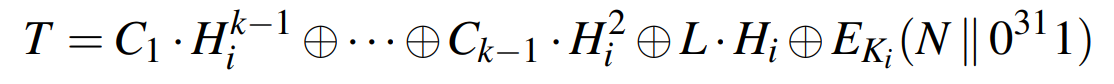
\includegraphics[scale=0.2]{equation_1.png}

which one arrives at by assigning $H_i$ to H and then substituting the result into the equation
$T = h \oplus E_{K_i}(N || 0^{31}1)$.
Note that we have fixed the number of the
ciphertext blocks to be k-1.
The resulting system of k equations in k unknowns will be:

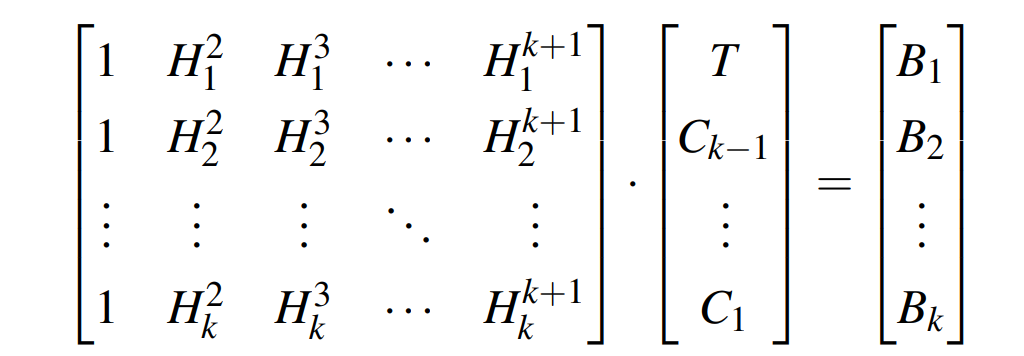
\includegraphics[scale=0.2]{system_of_equations_1.png}

where $B_i = (L \cdot H_i) \oplus E_{K_i}(N || 0^{31}1)$.
We can optimize this system of equations and transform it to a system which can be solved in time $O(k^2)$ and space $O(k)$.
Please refer to \cite{cryptoeprint:2020:1491} for details.

\hfill \break

For such a system to be solvable, there have to be rows that are linear combinations of other rows.
Since each row is increasing powers of a random field element (i.e., the hash key) this
dependence between rows should be rare as long as the
block cipher acts like an ideal cipher.
For explanations please refer to \cite{cryptoeprint:2020:1491}.

an example of key multi collision algorithm on the AES-GCM scheme:
\\

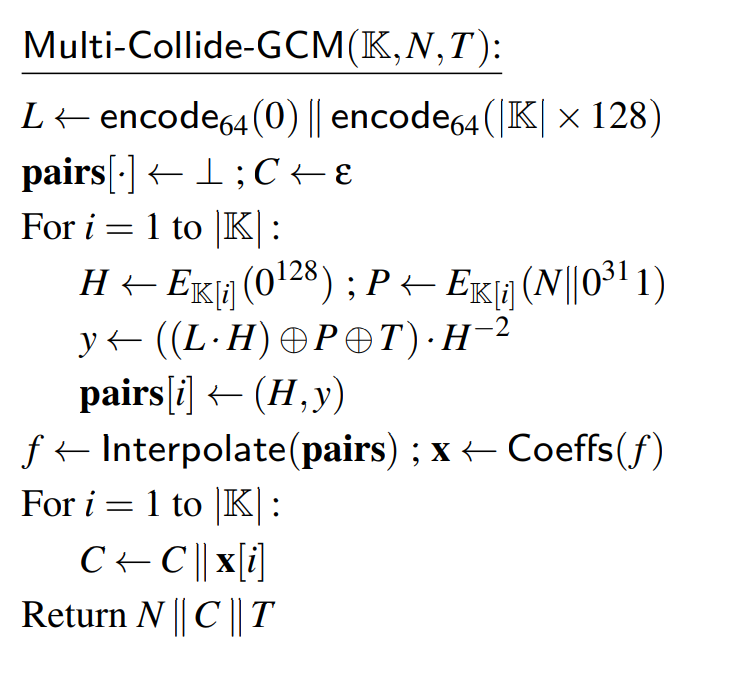
\includegraphics[scale=0.3]{mkca_aes_gcm.png}